

\documentclass[a4paper,12pt,oneside]{report}
\usepackage{formai_kovetelmenyek}

\hypersetup{
	pdfauthor={Biró Dávid},
	pdftitle={Webalapú ER modellező}
}

\lstset{
	basicstyle = \ttfamily\footnotesize
	,breaklines = true
	,prebreak   = \raisebox{0ex}[0ex][0ex]{\ensuremath{\hookleftarrow}}
	,extendedchars = true
	,literate={á}{{\'a}}1 {ó}{{\'o}}1 {é}{{\'e}}1 {í}{{\'i}}1 {ő}{{\~o}}1 {ö}{{\"o}}1 {ű}{{\'u}}1
}

\hyphenation{Google}

\title{Webalapú ER modellező}
\author{Biró Dávid}
\date{}

\widowpenalty=400
\clubpenalty=400

\graphicspath{{./resources/}}

\setcounter{secnumdepth}{4} %szamozza a subsubsection-oket is
\AtBeginDocument{\addtocontents{toc}{\protect\pagestyle{empty}}} %ezzel erem el, hogy a tartalomjegyzek ne kapjon oldalszamot
\AtBeginDocument{\addtocontents{tod}{\protect\thispagestyle{empty}}}

\begin{document}
\setcounter{chapter}{1}

\pagestyle{empty}
\newpage
%------------------------------------------------------------------
% külsõ kötéstábla
{
    \begin{center}
    \vspace*{5cm}
    {
        \Huge SZAKDOLGOZAT}\\
        \vspace*{10cm}
        {\LARGE Biró Dávid}\\
        \vspace*{3cm}
        {\LARGE 2019}
    \end{center}
}
\pagebreak
\newpage
% címoldal
\begin{center}
{
    \Large Pannon Egyetem\\
    Műszaki Informatika Kar\\
    Rendszer- és Számítástudományi Tanszék
    \vspace*{3mm}\\
    Programtervező informatikus BSc szak
}
    \vspace*{2cm}\\
    {\LARGE \bf SZAKDOLGOZAT}
    \vspace{3cm}\\
    {\LARGE\bf Webalapú ER modellező}
    \vspace{3cm}\\
    {\large Biró Dávid}
    \vspace{6cm}
    \\
    {\large Témavezető: Machalik Károly}
    \vspace{1cm}\\
    {\large 2019}
\end{center}
\normalsize
% címlap vége
\newpage
Ide jön az eredeti vagy a fénymásolt feladatkiírás.
\newpage
\begin{center}
\section*{Nyilatkozat}
\end{center}

Alulírott Biró Dávid diplomázó hallgató kijelentem, hogy a szakdolgozatot a Pannon Egyetem Rendszer- és Számítástudományi Tanszékén készítettem Programtervező informatikus BSc szak (BSc in Computer Engineering
) megszerzése érdekében.

Kijelentem, hogy a szakdolgozatban lévő érdemi rész saját munkám eredménye, az érdemi részen kívül csak a hivatkozott forrásokat (szakirodalom, eszközök, stb.) használtam fel.

Tudomásul veszem, hogy a szakdolgozatban foglalt eredményeket a Pannon Egyetem, valamint a feladatot kiíró szervezeti egység saját céljaira szabadon felhasználhatja.
\vspace{0.5cm}
\begin{flushleft}
{Veszprém, 2019. május 10.\\}
\end{flushleft}

\begin{flushright}
{Aláírás \vspace{4cm}}
\end{flushright}

Alulírott Machalik Károly témavezető kijelentem, hogy a szakdolgozatot Biró Dávid a Pannon Egyetem Rendszer- és Számítástudományi Tanszékén készítette Programtervező informatikus BSc szak (BSc in Computer Engineering) megszerzése érdekében.

Kijelentem, hogy a szakdolgozat védésre bocsátását engedélyezem.\\

\begin{flushleft}
{Veszprém, 2019. május 10.\\}
\end{flushleft}

\begin{flushright}
{Aláírás}
\end{flushright}
%A tartalomjegyzék:
\newpage
\begin{center}
\section*{Köszönetnyilvánítás}
\end{center}
\begin{justify}
Köszönettel tartozom Machalik Károlynak, aki segített a szakdolgozat formai követelményeinek betartásában, valamint a szakdolgozat előadási módjának fejlesztésében.

Köszönettel tartozom a Phoenix framework fejlesztőinek, hogy biztosítottak egy hasonló kódgenerátort, ami alapján ez a szakdolgozat létrejöhetett.

Végül köszönettel tartozom Öze Csillának és a családomnak, az állandó támogatásért.


\end{justify}
\newpage

\sectionfont{\centering\large\sffamily}

\begin{center}
\section*{\textbf{\Large \MakeUppercase{\textrm{Tartalmi összefoglaló}}}}
\end{center}


\begin{justify}
A szakdolgozat témája egy webalapú ER modellező készítése. Ezen belül is egy megfelelő eszköz biztosítása a rapid-prototyping fejlesztési módszer segítésére, első sorban web alapú alkalmazásokhoz.

A webes alkalmazások nagy része tartalmaz olyan közös elemeket, amelyek lehetővé teszik, hogy akár kevés információval is, de generálhatóak legyenek.

A szakdolgozatban bemutatott program egy módosított Entity Relationship modellt használ a legenerálandó erőforrások definiálására. Ehhez a modellhez biztosít egy tervező felületet, hogy a generátor használata a lehető legkényelmesebb, és leggyorsabb legyen.

Az átláthatóság érdekében a generátor sablonjai csomagokba lettek rendezve, melyeken belül találhatók továbbá a követelményfájlok, amelyek leírják, hogy milyen követelményeknek felelhet meg az aktuális sabloncsomag. Ezen követelmények mindegyike opcionális, így lehetőséget ad arra is hogy a nem kívánt funkciókat ne vigye bele a rendszerbe.

A program  biztosít lehetőséget saját sabloncsomagok létrehozására és a meglévők módosítására is.

A kódgenerátorok nagy hátránya, hogy az absztrakt megfogalmazás már nem módosítható anélkül, hogy a kódot újra kelljen generálni. A szakdolgozat keretében elkészített alkalmazás ezen nem változtat, viszont ad egy megoldást erre a problémára a git verziókezelő rendszer használatával. 

A program segítségével lehetőség nyílik arra, hogy ne csak egyszerű, hanem komplex szerver- és ezzel együtt kliens oldali kódokat tudjunk generálni, ezzel utat nyitva a jól strukturált, könnyen módosítható, webes alkalmazások felé.
\end{justify}

\vspace{2cm}

{\bf Kulcsszavak:} {\it scaffolding, web, kódgenerátor, rapid-prototyping, ER, modellező}

\newpage
\begin{center}
\section*{\textbf{\Large \MakeUppercase{\textrm{Abstract}}}}
\end{center}



\begin{justify}
This thesis is for creating a web-based ER modeller and the right tool for fast-prototyping based development for websites at first.

The most of the web-pages share common properties that make them possible to be generated with just a little information. By this idea, the software introduced in this thesis is a code generator, which uses a modified entity-relationship model for the definition of generable resources. For this model, the application provides a designer interface in order to ease the use of the generator.

Respecting the readability the templates of the generator had been organized into packages. In packages, requirement files can be found, which shows, which requirements are suitable for the template package. All requirements are optional, so it gives the ability to skip unnecessary functionalities from the new system. In order to convince the users, the generator supports adding own template packages and modifying the existing ones.

So far, the code generators share a common disadvantage: The abstract definition can not be changed without re-generating the entire code. The software introduced in the thesis does not make it different but shows a solution using the Git version control system. 

By the help of this application, opportunities open up for generating not just simple but complex server- and client side codes, with opening gates to the well-structured, easily modifiable web applications. 
\end{justify}



\vspace{2cm}

{\bf Keywords:} {\it  scaffolding, web, code, generator, rapid-prototyping, ER, modeller}
\newpage

\allsectionsfont{\sffamily\large} %14pt
\subsectionfont{\sffamily\normalsize} %12pt
\subsubsectionfont{\sffamily\normalsize} %12pt

%--------------%------------------------------------------------------------------
\pagenumbering{gobble} %ne legyen oldalszamozas a tartalomjegyzek oldalon
%\listoftodos

\renewcommand{\thefigure}{\arabic{figure}}

\setcounter{tocdepth}{3} %subsubsection-ok is latszodjanak
\thispagestyle{empty}
\tableofcontents
\pagebreak

\pagenumbering{arabic} %legyen oldalszamozas
\setcounter{page}{1} %innentől indul az oldalszámozás
\pagestyle{plain}
\fancyhead[C]{\rightmark}
\fancyfoot[R]{\thepage}
\section{Motiváció}
\subsection{Egy sikertelen megrendelés története}


\begin{justify}
	Egy webáruház készítésére kaptam megrendelést. A követelmények nem voltak teljesen ismertek, és a legtöbb csak a fejlesztés során derült ki. Annak érdekében, hogy a weboldal gyorsan elkészüljön, komponens alapú fejlesztést alkalmaztam, azaz az első lépés a megfelelő komponens kiválasztása volt.

	Mivel a webáruházak körében elterjedt a WooCommerce, ezért a döntésem is amellett állt. A WooCommerce egy plugin a Wordpress tartalomkezelő rendszerhez, amely az eredetileg blogokhoz szánt rendszert kiegészíti úgy, hogy webáruház lehessen az amúgy általános célú blogrendszerből.

	A fejlesztés első szakaszában még látszólag előnyös volt. Az ügyfél hamar láthatott egy működő webáruházat, azonban a később érkező specifikációk miatt rá kellett jönnöm, hogy nem ez volt a legjobb választás. 

	Az ügyfél a legkisebb dolgokat is megszerette volna változtatni, azonban a rendszer ezekre nem adott lehetőséget. Ekkor váltani már költséges volt, ezért kénytelen voltam módosítani a rendszer alapvető funkcióit, ellehetetlenítve így a frissítés lehetőségét. A fejlesztést az is megnehezítette, hogy a kód azon részeihez nem volt dokumentáció, így egy ilyen módosítás akár nem megfelelő működést is eredményezhet. Így is lett. Az így beletett funkciók valamikor működtek, valamikor nem. Emellett a nem megfelelő architektúra miatt sebességbeli komplikációk léptek fel. Hosszas látszólag sehova nem haladó egyezkedések miatt, amikor már a projekt nagyon csődösnek lett ítélve, elkerülhetetlen volt a vége. 

	Egy lehetséges megoldás lett volna a megfelelő komponens kiválasztása a projekt kezdeti stádiumában. Azonban ez a választás nem tud alapulni megfontolt döntésen anélkül, hogy ismernénk a pontos követelményeket. Egy másik lehetséges megoldás lehet az alkalmazás fejlesztése kész Content Management System (CMS) nélkül. Ez a megoldás ad a lehető legjobban strukturált szoftvert az adott funkcionális követelményekre. A jó struktúra miatt feltehetően sebességre is jobban optimalizáltabb, azonban egyben ez a legdrágább is.
\end{justify}

\newpage
\subsection{Miért ne használjunk nagy komponenseket, mint kész tartalomkezelő rendszereket}

\begin{justify}
	A komponens alapú fejlesztés a programozási módszertanok egyike. A lényege, hogy a program nagy részét kész komponensekből építjük fel, aztán a komponenseket megpróbáljuk minél jobban az igényekre szabni, ha ezeket nem tudja a komponens teljesíteni akkor meg lehet próbálni a követelmények módosítását, amennyiben az ügyfél elég rugalmas erre. Ha nincs megfelelő komponens azt le kell fejleszteni. \cite{website:component_based_development}

	A nagy komponensek előnye, hogy költségkímélőbb, mint ugyanazt a funkcionalitást újból megvalósítani.

	Hátrányait minden komponensre egyedileg lehet megfogalmazni, de általánosságban legtöbb komponens dokumentációja csekély, a képességeik nagyon limitáltak, és továbbfejlesztésre nem adnak elég lehetőséget. Előfordul, hogy túl sok felesleges funkciót is tartalmaznak. Ebben az esetben sokszor az automatizáltság miatt nehéz az egyedi funkciók hozzáfejlesztése.

	Az egyedi funkciók hozzáfejlesztése fontos, ugyanis az üzleti követelmények gyorsan változhatnak olyan irányba, ami egy nem előrelátható limitáltságot hoz elő a komponenseknél. Célszerű nem nagy komponenseket választani, hogy a cseréjük ne legyen költséges. Nagy komponensnek számít egy tartalom kezelő rendszer, mint például a WordPress. A tartalom kezelő rendszerek helyett, lehet használni keretrendszereket, amikhez csak kisebb komponensek érhetőek el, és közülük kevés biztosít felesleges funkcionalitást, valamint a cseréjük is egyszerűbb. \cite{website:cms_or_fw}

\end{justify}

\newpage
\subsection{Miért jó a “Rapid Prototyping”}

\begin{justify}

	Az ügyféltől nem szabad többet várni, minthogy megmondja, hogy jó-e így a program, vagy sem. A Rapid Prototyping egy olyan programozási módszertan, aminek a lényege, hogy egy gyors prototípus segítségével a nem ismert követelményeket felderítsük. A gyors prototípus készítésére megfelelő eszközök szükségesek, ilyenek lehetnek például kódgenerátorok, terminálos kis eszközök vagy akár tervező programok. \cite{website:rapid_prototype}

	A Rapid Prototyping programozási módszer fejlesztő barát mert a programozó a fejlesztésre fókuszál és nem a komponensek integrációjára, másrészt segít a fejlesztőnek is a megfelelő projekt struktúra kialakításában, hiszen a prototípus még jelentősen módosítható.

	A módszer egy jól strukturált, könnyen továbbfejleszthető minimális programot eredményez, ami teljesíti a szükséges követelményeket. A bővíthetősége jól illeszkedik a változó üzleti igényekre. 

	Habár a módszer előnyeit tekintve nagyon kedvező lehet, legtöbbször mégis inkább az aktuális igényeknek megfelelő, kész rendszereket integrálnak egy új fejlesztése helyett. Ez egyrészt azért lehet, mert egy új rendszer fejlesztése látszólag költségesebb, és az első értékelhető eredményt jóval később kapja meg az ügyfél. Weboldalaknál a hasonlóságaik miatt, ez a folyamat könnyen felgyorsítható egy erre specializálódott eszköz segítségével.

\end{justify}

\newpage
\subsection{A megfelelő eszköz a Rapid Prototyping fejlesztési módszertan segítésére, weboldalakhoz }

\begin{justify}

	Kódgenerátorok alkalmazása jelentősen tudja növelni a fejlesztési sebességet. Anélkül, hogy a komponensek integrációjával törődnénk, a generált kód már tartalmazhat integrált apró komponenseket és - ha esetleg másként szeretnénk használni - egyben példakódot is a használatukra. A megfelelő eszköz egy olyan kódgenerátor, ami már egyben stabil és felhasználásra kész programkódot generál, de megengedő annyira, hogy kikapcsolhatóak a nem kívánt funkciók generálása a kívántak megtartásával.

    A weboldalak nagy része csupán csak egy tartalom kezelő rendszer. Gondoljunk egy egyszerű blog rendszerre, ahol van 1 oldal a bejegyzések listázására, és kell lennie egy admin felületnek, ahol ezeket a bejegyzéseket menedzselik. Ezek az oldalak általában a tartalmat egyszerű űrlapokkal kezelik (pl.: hozzáadás, szerkesztés, törlés). Ezek az űrlapok építik fel az egész webes alkalmazást, az adatbázis rétegtől a kinézetig, de teli vannak olyan közös elemekkel, amelyek lehetővé teszik, hogy az űrlapok, kevés információval is generálhatóak legyenek. Ezekhez az oldalakhoz általában elég egy erőforrás név (pl.: bejegyzés), az erőforrás attribútumai (pl.: a bejegyzés neve) és a típusa (pl.: szöveg). 
    
    \label{sec:abstraction_level}
	A legegyszerűbb tartalom kezelő rendszer ennyi adatból már generálható, azonban a komplexebb weboldalaknál több erőforrás is van, és ezek kapcsolódnak is egymáshoz (pl.: a felhasználónak van több bejegyzése). Ha belevesszük a kapcsolatokat is az absztrakcióba, akkor a lehetőségek tárháza nyílik meg. Ha az ``egy a sokhoz” (egy egyedhez több egyed tartozik) kapcsolatot nézzük, akkor létrejöhetnek olyan oldalak, amik ezt a kapcsolatot felhasználják:

	\begin{itemize}
		\item csak a felhasználó bejegyzéseinek a megjelenítése
		\item felhasználók és bejegyzések pároztatása
		\item bejegyzés hozzáadása (felhasználóként)
	\end{itemize}

	Ha létezne egy olyan kód generátor, ami ezen absztrakciónak a lehetséges kimeneteit legenerálja, akkor már szinte csak a frontend-el kellene foglalkozni. (Frontend-nek hívjuk az applikáció azon részét, ami a felhasználónak látható felület megjelenítéséért felelős.) 

	Az egyedi elemeket - mint a felhasználói felület kinézete - nem tudja kiváltani, de példakódot biztosíthat hozzá.

	Egy kódgenerátornál fontos az is, hogy gyorsan el tudjon indulni, és az absztrakció megfogalmazását egyből megkezdhessük. Webfejlesztés során a terminál kulcsfontosságú elem, és általában nyitva van a különböző eszközök miatt (pl: Node Package Manager (NPM)). A megnyitott terminál általában az aktuális projekt könyvtárába van lépve, ami kiváló lehetőséget ad arra, hogy innen indítsuk el az ezköszt. Egy jó kódgenerátornak érdemes kezelnie egy bemenő paramétert arra a célra, hogy jelezze, hogy hol induljon el (pl: a Visual Studio Code biztosít lehetőséget arra, hogy könnyen elindítsuk az aktuális mappában: 'code .') 

	Fontos, hogy az absztrakt megfogalmazásból minél több kódot lehessen generálni, ezzel levéve a terhet a programozók válláról. Az absztrakciónak a félúton kell lennie a specifikus és általános között, hogy sokatmondó legyen a modell, de egyben egyszerű is.


\end{justify}

\newpage
\subsection{Hasonló technológiák}
\subsubsection{QuickAdminPanel a Laravel keretrendszerhez}

\begin{justify}

	A Laravel egy PHP alapú keretrendszer, ami MVC (Model View Controller) tervezési mintát követ, ezzel lehetőséget adva dinamikus weboldalak jól strukturált elkészítéséhez. 

	A QuickAdminPanel egy admin panel generátor a Laravel keretrendszerhez. A generátor internetes, és lokálisan nem elérhető. A generált állományokat le kell tölteni, és úgy integrálni a rendszerbe. A generátor az adatbázis rétegről a nézet rétegig mindent generál, így biztosítva a lehetőséget arra, hogy egy erőforrást lehessen listázni, hozzáadni, szerkeszteni és törölni. Kezeli az erőforrások kapcsolatát is, így akár komplexebb oldalakat is képes generálni.

	Hátránya, hogy nem elég átlátható a felület. Új erőforrás létrehozása közben nem látszódnak a hozzá kapcsolható erőforrások. Bizonyos részei fizetősek, és nem biztosít elég segítséget az integrációra. A zártsága miatt nem kiegészíthető, és csak a Laravel keretrendszerhez érhető el.

\end{justify}

\newpage
\subsubsection{A Phoenix keretrendszer beépített generátora}

\begin{justify}
	A Phoenix az egy Elxir nyelven írt, a laravelhez hasonló MVC felépítésű keretrendszer. Az elixir egy erlang alapú funkcionális nyelv. 

	A Phoenix biztosít egy CLI eszközt a keretrendszer egyes lehetőségeinek automatizálására, így egy egyszerű generátort is. A generátor csak erőforrás listázást, szerkesztést, hozzáadást, törlést, valamint egy külön oldalt biztosít egy erőforrásnak. Kapcsolatokat támogatja, de a generált felületen a idegen kulcsokat csupán számként kezeli. A használata elég egyszerű: 

	\begin{figure}[h]
		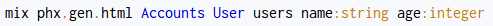
\includegraphics[width=\textwidth]{contents/images/mix_phx_gen_html.png}
		\caption{Példa a használatra}
		\label{fig:mix_phx_gen_html}
	\end{figure}

	Hátránya, hogy egyszerre csak egy erőforrás generálására alkalmas, és viszonylag keveset segít.

\end{justify}

\newpage
\section{Rendszerterv}
\subsection{Tervező}
\subsubsection{Az Entity Relationship modell}

\begin{justify}

	Egy kódgenerátornál fontos az is, hogy miképp adjuk át a szükséges információkat a projektről. Az egyik lehetőség a Command Line Interface (CLI) használata, ami gyors, de meg kell tanulni a használatát, valamint sok információ átadására nem alkalmas. Éppen ezért egy grafikus megfogalmazás előnyösebb lehet. Az \hyperref[sec:abstraction_level]{előzőekben} említett absztrakciós szintnek az Entity Relationship (ER) modell adattípusokkal kiegészített változata pont megfelel.

	% from: https://medium.com/omarelgabrys-blog/database-modeling-entity-relationship-diagram-part-5-352c5a8859e5
	\begin{figure}[h]
		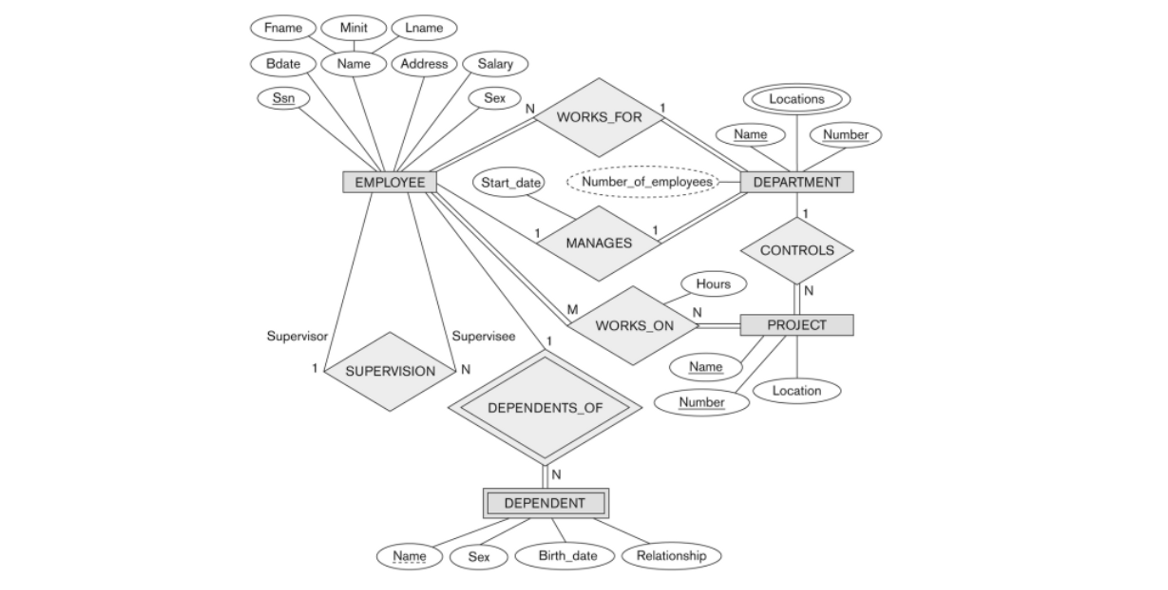
\includegraphics[width=\textwidth]{contents/images/ermodell_example.png}
		\caption{Példa az Entity Relationship modellre \cite{website:example_of_er} }
		\label{fig:ermodell_example}
	\end{figure}

    Az ER modell a nevéből is következtethetően entitásokat és azok kapcsolatait modellezi. Az entitás téglalap alakú, és egy elemet reprezentál (pl: egy felhasználó a felhasználókból). A rombusz egy kapcsolatot jelöl két entitás között. Itt 3 féle lehet:

    \begin{itemize}
        \item Egy az egyhez (1db $A$ entitáshoz maximum 1db $B$ entitás tartozhat).
        \item Egy a sokhoz (1db $A$ entitáshoz több $B$ entitás is tartozhat).
        \item Sok a sokhoz (1db $A$ entitáshoz több $B$ entitás is tartozhat, és 1db $B$ entitáshoz több $A$ entitás is tartozhat).
    \end{itemize}
\end{justify}
\newpage
\begin{justify}
	Az ER modell különbséget tesz két fajta kapcsolat között:
    
    \begin{itemize}
        \item Erős kapcsolat (a kapcsolat megléte kötelező).
	    \item Gyenge kapcsolat (a kapcsolat megléte opcionális).
    \end{itemize}

	Minden entitásnak, és a kapcsolatnak lehetnek attribútumaik (pl: felhasználónak a felhasználónév). Az attribútumoknak a következő típusai vannak: 

	% from:  Fogarassyné Vathy Ágnes - Adatbáziskezelő rendszerek I. - Egyed-kapcsolat modell
	\begin{figure}[H]
		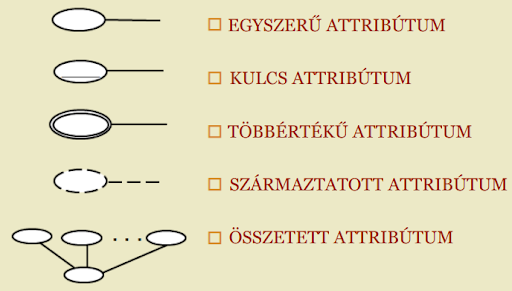
\includegraphics[width=\textwidth]{contents/images/ermodell_attributes.png}
		\caption{Az attribútumok típusai \cite{book:example_er_attr} }
		\label{fig:ermodell_attributes}
	\end{figure}

	A modellt eredetileg arra tervezték, hogy akár az ügyfél által is validálható legyen a terv, így használata nagyon egyszerű, és jól dokumentálja a projekt szerkezetét. Hasonló absztrakció megfogalmazására képes az adatbázis logikai modell, ahol a kapcsolatok már kulcsokkal vannak ábrázolva, de az olvashatósága sokkal nehezebb, ami miatt az entity relationship modell a legmegfelelőbb a feladatra. 

\end{justify}

\newpage
\subsubsection{Létező Entity Relationship modell tervezők}

\begin{justify}

	Egy tervezőnél létfontosságú, hogy mindent gyorsan és egyszerűen meg lehessen benne tervezni. Az alábbi ábra az alapvető lépéseket hasonlítja össze különböző tervezőprogramoknál.

	\begin{table}[H]
		\centering
		\begin{tabular}{|l|l|l|l|l|}
			\hline
			Eszköz & \begin{tabular}[c]{@{}l@{}}Egyed\\ létrehozása\end{tabular} & \begin{tabular}[c]{@{}l@{}}Attribútum\\ hozzáadása\end{tabular} & Összekapcsolás & Törlés \\ \hline
				erdplus.com & 2 & 4 & 3 & 2 \\ \hline
				draw.io & sok & sok & túl sok & 2 \\ \hline
				gliffy.com & sok & sok & túl sok & 2 \\ \hline
				sqldbm.com & 3 & sok & 4 & 3 \\ \hline
				smartdraw.com & 2 & sok & túl sok & 2 \\ \hline
		\end{tabular}
	\end{table}

	A mérésnél 1 lépésnek számított a kattintás, az elnevezés, a húzás, a billentyű lenyomása (ha nem szöveg írásra használtuk) és a szöveg írása. A mért adatok azóta változhattak. 

	Az összehasonlított rendszerek közül egyik sem volt felhasználóbarát. A sok panel miatt a diagramból kevés látszott. Az egyes elemek rendezése gondot okozott. Előfordult, hogy a kapcsolatok nem frissültek az egyedek mozgatása után.

\end{justify}

\newpage
\subsubsection{Egy jobb tervező terve}

\begin{justify}

	A legtöbb ER Modell tervező használhatatlan a kisebb képernyőkön, a sok képernyőterületet foglaló panelek miatt. Annak érdekében, hogy minél többet lássunk a modellből, a terv egy olyan ER modellező, ami majdnem teljesen panel mentes. 

	A mozgatás segítésére az attribútumok az entitások része, így mikor egy entitást mozgatunk, akkor mozgatjuk az attribútumait is. Az entitások közötti kapcsolat frissül, ha valamelyik entitás pozíciója a kapcsolatban megváltozik. Az objektumok elrendezése félig automatikus, ami azt jelenti, hogyha az elemek túl közel vannak egymáshoz, látszólag maguktól eltávolodnak.

	A gyors modell tervezéséhez, minden felhasználói akció lehetőleg csak 1 lépést vesz igénybe.

	A felhasználók meggyőzéséért egy modern, minimalista stílusú felülettel rendelkezik, jól látható elemekkel. A kapcsolatok leegyszerűsítése érdekében a kapcsolat $1..n$, $n..m$, stb... jelölések helyett grafikusan ábrázolja a kardinalitást, a következő módon:

    \begin{figure}[h]
        \centering
		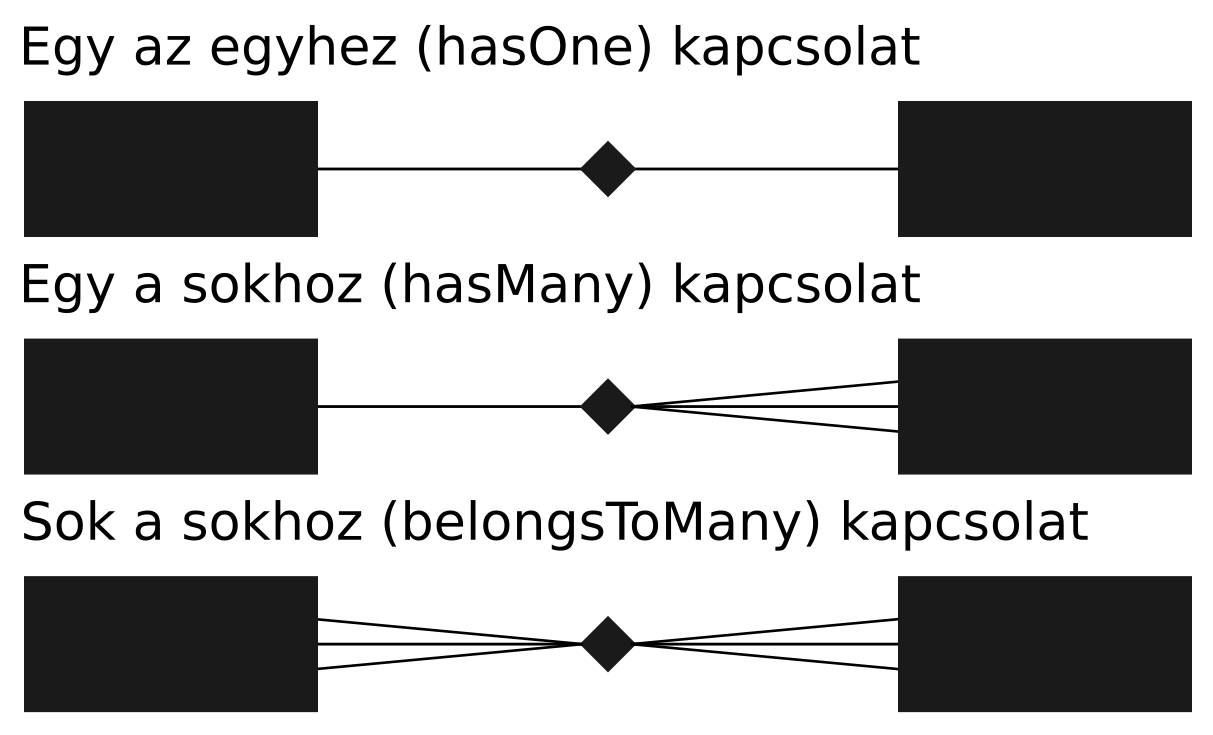
\includegraphics[width=12cm]{contents/images/simplified_relations.png}
		\caption{Leegyszerűsített kapcsolatok}
		\label{fig:simplified_relations}
	\end{figure}

	Ezen grafikus reprezentáció kényelmesebben olvasható, ugyanakkor, ha szükség van kötelező és opcionális kapcsolatok megfogalmazására, ugyanúgy jelölhetjük őket vastag, illetve vékony vonallal. 

\end{justify}

\newpage
\subsubsection{A Modell kiegészítései }

\begin{justify}

	Ahhoz, hogy a modellt használni lehessen webes alkalmazások generálására, szükséges pár módosítást elvégezni rajta. Az egyik ilyen módosítás az attribútumok típusokkal való kiegészítése (pl.: name helyett name : string). A típusok szükségesek az űrlapok elkészítéséhez. A típusok adják meg azt, hogy milyen bemeneti mező szükséges az egyes attribútumok megadásához.

	Egy kész webalkalmazás mindig foglalkozik a bemenet validálásával. A validáláshoz szükséges információkat a típus nevében szükséges lehet jelölni (pl.: name : string[MIN=3, MAX= 15]).

	Ha az entitások nevei az angol nyelvben megszámlálhatóak, akkor az adatbázis táblát az entitás nevének többes számú alakja alapján el lehet készíteni. Azonban, ha nem megszámlálhatóak, akkor biztosítani kell egy lehetőséget, hogy kézzel beírható legyen. Egyes Object Relation Mapping (ORM) rendszerek alapból az entitás többes számú alakját használják a Repository réteg neveként. A Repository réteg nevét fel lehet használni az adatbázistábla nevéhez is. Így az entitás nevéhez meg kell adni egy kiegészítő nevet is, ami a több ugyanolyan entitással foglalkozó absztrakcióra fog utalni. (Pl.: Music : MusicRepository)

\end{justify}

\newpage
\subsection{Generátor}
\subsubsection{Példa egy egyszerű erőforrás kezelőre}

\begin{justify}

	Az egyszerűbb megértés érdekében, nézzünk egy példát egy erőforrás kezelésre. Legyen az erőforrás a bejegyzések egy blog rendszerben. Ebben az esetben szükség van egy Post nevű entitásra és pár alapvető attribútumra. Az egyik attribútum az ID, amivel azonosíthatjuk a bejegyzéseket, egy másik a Title, ami a bejegyzés neve, és egy harmadik a Content, ami a bejegyzés tartalma. Az ID típusa integer, a többi mind string. Ábrázolva a módosított ER modell segítségével, a következőképpen néz ki:

	\begin{figure}[h]
		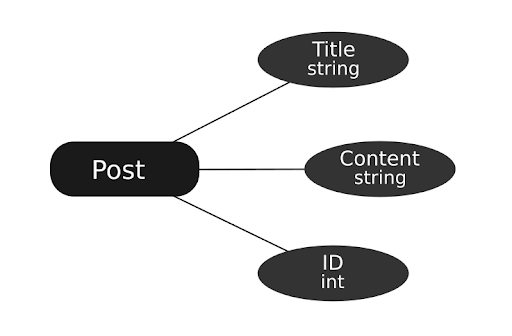
\includegraphics[width=\textwidth]{contents/images/post_ermodel.png}
		\caption{Egy bejegyzés modellje a kiegészített ER modellel ábrázolva}
		\label{fig:post_ermodel}
	\end{figure}

	Ránézésre a következő oldalak jutnak eszünkbe a modell kapcsán:

    \begin{itemize}
        \item Bejegyzések listázása.
        \item Bejegyzés hozzáadása.
        \item Bejegyzés módosítása.
    \end{itemize}

	Ezek az oldalak jelentik a követelményeket a rendszerrel kapcsolatban. Ahhoz, hogy ezeket létrehozhassuk, szükséges egy olyan sabloncsomag, ami ezeknek a követelményeknek eleget tud tenni. A sablonoknak vannak függőségeik, aminek célja, hogy a sablon funkcionalitásához szükséges egyéb sablonok is legenerálódhassanak.  Egy sabloncsomagon belül vannak követelményfájlok, amik leírják a követelményeket, és egy kezdő sablont biztosít minden egyes követelményhez, ami egy belépési pont a függőségi gráfban.

	\begin{figure}[h]
		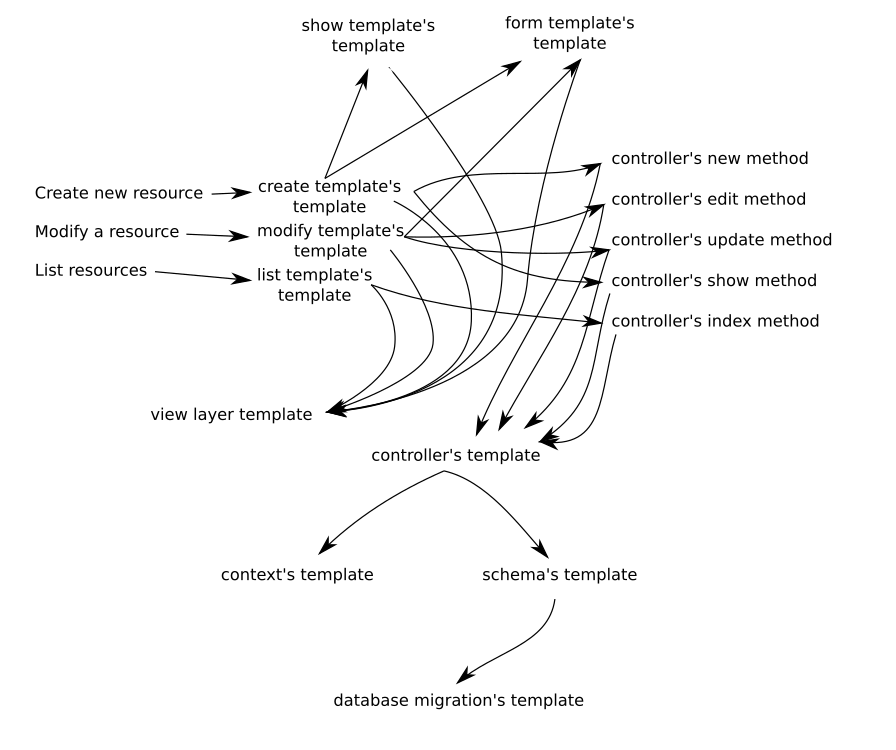
\includegraphics[width=\textwidth]{contents/images/dependecy_graph.png}
		\caption{Példa a függőségi gráfra}
		\label{fig:dependecy_graph}
	\end{figure}

	Az ábrán látható, hogy mennyi mindent kell létrehozni egy-egy entitás esetében. A gyakorlatban ez tovább bonyolódik. Opcionális követelmények esetében, egy-egy sablon nem feltétlen külön fájl létrehozására, hanem egy meglévő fájl módosítására szolgál. A fenti ábra is ábrázolja a controller több metódussal való kiegészítését. Gyakorlatban ez nem csak a controllernél jelent további bontásokat, hanem külön eset kell arra is, ha valaki nem szeretné listázni az egyes erőforrásokat, és emiatt új létrehozásakor ne ajánljon fel linket az összes mutatására, ugyanis az az oldal nem fog létezni.

	A függőségi gráf nem feltétlen feszítőfa. Lehetnek körkörös függőségek, többszörös hivatkozások is. A program szempontjából ezt kezelni kell oly módon, hogy a sablonnak átadott bemeneti adatok és a fájlnév kombinációja alapján a sablon maximum egyszer generálódjon le.

	A követelményfájlok megkapnak egy entitást, majd egy függvényben eldöntik, hogy arra az entitásra megvalósítható-e az aktuális követelmény. Ha megvalósítható a követelmény akkor az entitásból nyert adatok alapján (attribútumok, kapcsolatok), átadják az első sablonnak a sablon bemeneti paramétereit.

	A sablonok felépítésileg két részből kell, hogy álljanak:

    \begin{itemize}
        \item A sablon metaadatai.
        \item A sablon által generálandó kód.
    \end{itemize}

	A metaadatok dinamikus adatok, vagyis a bemenő paraméterként megkapott adatokból készül. Ezek írják le, hogy a sablont hova, milyen néven, milyen jogosultsággal kell legenerálni, illetve, ha meglévő fájl módosítására használjuk, akkor melyik fájl melyik szekciójába generálja és milyen művelettel (szekció cseréje, szekció előtt, szekció után). A metaadatok tartalmazzák a sablon egyes függőségeit is. 

	A sablon egy egyszerű szöveg, kiegészítve változókkal vagy a használandó sablon motor által biztosított nyelvi elemekkel.

	Ha egy sablonban megadott elérési út nem létezik, akkor a generátornak létre kell hoznia rekurzívan minden mappát és magát a fájlt is. Ha a megadott út módosítás céljából lett odaírva, de nincs olyan fájl, akkor a sabloncsomag függőségei rosszul lettek definiálva.

\end{justify}

\newpage
\subsubsection{Lehetséges jelentések különböző modellekre}
\begin{justify}

	A struktúrában nagyon sok mindenre lehet következtetni. Ha csak a struktúrát nézzük akkor 6 jól elkülöníthető eset létezik:

	\begin{itemize}
		\item Egy az egyhez kapcsolat.
		\item Egy a sokhoz kapcsolat.
		\item Sok a sokhoz kapcsolat.
		\item Rekurzív egy az egyhez kapcsolat.
		\item Rekurzív egy a sokhoz kapcsolat.
		\item Rekurzív sok a sokhoz kapcsolat.
	\end{itemize}

    Az egy az egyhez kapcsolat valamilyen adat kiegészítést jelent. Ha van pár attribútum, ami elég bonyolult ahhoz, hogy külön entitásként kezeljük, akkor erre az entitásra alkalmazhatjuk ezt a kapcsolattípust. 
    
    Egy felhasználó lakcíme jó példával szolgál. A lakcím sok elemből áll, és lehet, hogy a kitöltése nem is kötelező. Ekkor a felhasználó entitást összekapcsolhatjuk egy “egy az egyhez” kapcsolattal a lakcím entitáshoz. (Az Entity Relationship modellben erre külön vannak összetett attribútumok, gyakorlatilag a kettő megvalósítás között elhanyagolható különbség van.)

    Az egy a sokhoz kapcsolat, a leggyakrabban használt kapcsolati forma. Jó példa erre egy blog rendszer, ahol a bejegyzések alá lehet írni megjegyzéseket. Ezt a kapcsolatot “van sok” (angolul: has many) kapcsolatnak szokás hívni, amiatt, mert az A entitásnak van sok B entitása. Ebben az esetben a bejegyzésnek van sok hozzászólása.

    A sok a sokhoz kapcsolatra jó példa lehet a zenék és a stílusok kapcsolata. A modern zenéket már nehéz besorolni egy-egy stílusba, ugyanis több, mint egy igaz rájuk. Ugyanakkor, egy stílusra sem csak egy zene érvényes. Ilyenkor a zenéhez tartozik több stílus, a stílushoz pedig több zene. Elképzelhető egy olyan felület, ahol zenéket és stílusokat kell pároztatni. Talán gyakoribb példa, egy új zene beküldésekor a zenére jellemző stílusok kiválasztása.   

	A rekurzív kapcsolatoknak talán legritkább változata az egy az egyhez kapcsolat. Az ilyen kapcsolat egy láncolt listához hasonló kapcsolatot ír le. Ha egy adatbázis tekintetében nézzük, és egy táblára gondolunk, akkor az ilyen tábla elkülöníthető listákat írna le. Habár használatára nehéz példát találni, a megléte nem okoz gondot, viszont szintén kibővíti a lehetséges felületeket. 

	A rekurzív ``egy a sokhoz” kapcsolat egy fa szerkezetet ír le. A legjobb példa erre a részlegek felépítése. Egy nagy cégnél különböző részlegek lehetnek, akár elhelyezés szerint (Berlin, Veszprém, Bécs), de minden egyes részleghez tartozhat több kisebb részleg (fejlesztői, marketing, HR), és ezeken belül is még lehetnek apró részlegek. Ekkor elképzelhetőek különböző felületek: 

	\begin{itemize}
		\item Új részleg hozzáadása egy meglévőhöz. 
		\item Részlegek listázása fa szerkezetben. 
		\item Részleg áthelyezése
		\item stb...
	\end{itemize}

    A rekurzív sok a sokhoz kapcsolat gyakorlatilag egy általános gráf szerkezet. Ilyen lehet a szociális hálózat ábrázolása is. Ez alapján a következő felületek képzelhetőek el: 
    \begin{itemize}
		\item Kapcsolat hozzáadása. 
		\item Kapcsolat törlése.
		\item Új felhasználó létrehozása kezdeti ismerősök kiválasztásával.
		\item stb...
	\end{itemize}

	Fontos megemlíteni, hogy a generátor nem korlátozódik relációs adatbázisokra. Minden implementáció a sablonokon múlik. Így, ha célszerű, a sablon használhat akár gráf adatbázisokat is.   

	Nem csak a struktúrából lehet következtetni az egyes legenerálandó részekre, hanem attribútumok típusaiból, neveiből, valamint entitások neveiből is. Például, ha egy entitás attribútumának a neve created\_at és dátum típusú, akkor lehet feltételezni, hogy létrehozáskor ezt a mezőt az aktuális dátummal kell feltölteni. 

	Egy másik jó példa a User entitás, aminek megléte jelenthet bejelentkezést, regisztrációt és egyéb legenerálandó részeket is.

	Típusoknak bevihettünk nem megszokott típusokat is (pl.: image, audio, video). Ezekből szintén lehet következtetni még sok felületre (pl.: feltöltési lehetőség).

\end{justify}

\newpage
\subsubsection{Módosíthatóság}

\begin{justify}


    A kódgenerátorok legnagyobb hátránya, hogy generálás után, az absztrakt definíció nem módosítható anélkül, hogy a kódot újra ne kellene generálni. Egy projekt elején nem tudhatjuk az összes követelményt, ezért csak egy részét tudjuk legenerálni, amit utána módosítunk. Később ki fognak derülni más-más eltérő jellegű igények is, amit szintén generálni szeretnék, majd ismét módosítani. Szerencsére a Git verziókezelő erre a feladatra tökéletes. 
    
    A Git biztosít lehetőséget arra, hogy bizonyos funkcióknak a verzióit egy másik szálon vezéreljük. Ezeket a szálakat ágaknak (angolul: branch) hívják. Az ágakat egymásba lehet egyesíteni, ilyenkor annak az ágnak a módosításait amelyiket éppen beleegyesítünk az aktuális ágba, összefésüli, és az újakat beeszközöli. Ha az egyesítésnél komplikációk lépnek fel, akkor ezeket egyesével meg kell oldani. 

	A Git meglétét nyugodtan lehet feltételezni, hiszen csekély számú kivételtől eltekintve minden fejlesztő, minden projektet már a Git segítségével verzió-kezel.

	A módszer a módosítás lehetőségére a következő:


    \begin{figure}[H]
        \centering
		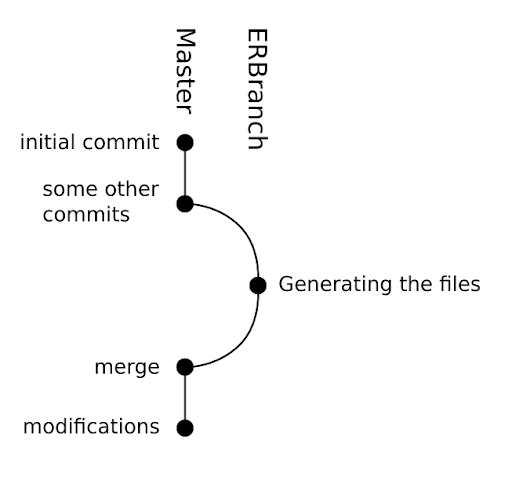
\includegraphics[width=12cm]{contents/images/git_first.png}
		\caption{Git ágak az első generálás után}
		\label{fig:git_first}
	\end{figure}

	A generátornak megadott generálási helyen feltételezzük, hogy a projekt már egy Git repository-ként inicializálva lett. A generálás során, a generátor létrehoz egy másik ágat ERBranch néven. 

	\begin{lstlisting}[language=GitBash]
	[generátor ]$ git checkout -b ERBranch 
	\end{lstlisting}

    Ezt az ágat csak a generátor használhatja. Generáláskor a generátor erre az ágra hozza létre a fájlokat. 
    
    Ahhoz, hogy ez egy visszaállítható állapot legyen, a változásokat elkövetjük. 

	\begin{lstlisting}[language=GitBash]
	[generátor ]$ git commit -a -m ‘Generation is succeded ’
	\end{lstlisting}

	A felhasználónak csak annyi dolga van, hogy visszamenjen arra az ágra, amelyikből az ERBranch ág leágazott, és egyesíti az ERBranch ág módosításaival.

	\begin{lstlisting}[language=GitBash]
	[felhasználó ]$ git checkout [-b] master
	[felhasználó ]$ git merge ERBranch
	\end{lstlisting}

	Az egyesítés közben felléphetnek konfliktusok (Git conflict), amit az egyesítéshez meg kell oldani. Egyesítés után készen áll a program a módosításra alacsony szinten.

    A fejlesztés során fény derülhet arra, hogy a modellt ki kell még egészíteni. Szerencsére a generátor erre is ad lehetőséget. 
    
    Nagyon fontos, hogy a lokális repository tiszta legyen, azaz minden hozzáadott módosítást véglegesíteni kell előtte:

	\begin{lstlisting}[language=GitBash]
	[felhasználó ]$ git commit -a -m ‘some message ’
	\end{lstlisting}

	Ezt követően a generátort újra lehet alkalmazni. A generátor ilyenkor már a meglévő ERBranch ágra megy át, és visszaállítja az azon lévő utolsó verziót.

	\begin{lstlisting}[language=GitBash]
	[generátor ]$ git checkout ERBranch
	[generátor ]$ git revert THE_LAST_COMMIT
	\end{lstlisting}

	Ekkor a generátor újragenerálja az egész projektet, de a Git szempontjából ez csak egy változtatásnak fog tűnni, amit szintén véglegesít. 

	\begin{lstlisting}[language=GitBash]
	[generátor ]$ git commit -a -m ‘Generation is succeded ’
	\end{lstlisting}

	Ismét visszatérünk az előző ágra, és egyesítjük azt az ERBranch nevű ággal, hogy megkapjuk a generátor módosításait. 

	\begin{lstlisting}[language=GitBash]
	[felhasználó ]$ git checkout master
	[felhasználó ]$ git merge ERBranch
    \end{lstlisting}
    
    Ekkor az ágak az alábbiak szerint fognak alakulni: 
	\begin{figure}[H]
		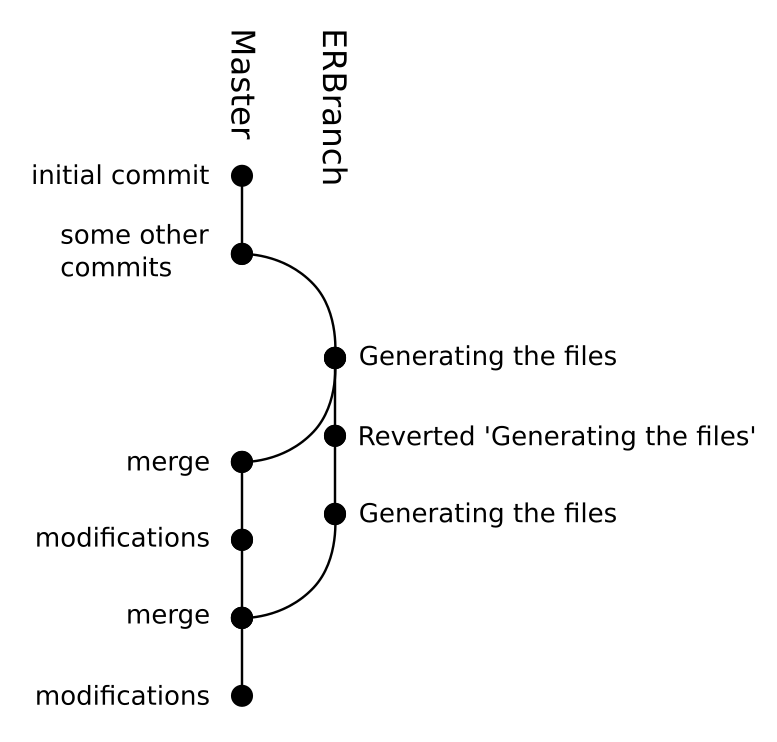
\includegraphics[width=\textwidth]{contents/images/git_second.png}
		\caption{Git ágak a modell módosítása után}
		\label{fig:git_second}
	\end{figure}

\end{justify}

\newpage
\subsubsection{A nagy sablonválaszték elérése}

\begin{justify}

	A sablonok a generátor szerves részei. Ha nincsenek sablonok, akkor a generátor használhatatlan. Éppen ezért, az új sablon létrehozása a lehető legkevesebb tanulást igénybe vevő megoldásnak kell lennie. 

	A dinamikusság és a kevés tanulás elérése érdekében a sablonoknak egy jól ismert programozási nyelven kell íródniuk. A Stack Overflow 2018-as felmérése szerint, a legismertebb programozási nyelv a JavaScript. \cite{website:most_known_language} A JavaScript-et nem csak emiatt érdemes használni, hanem mert van hozzá interpeter, és a sablonok gépi kódra fordítás nélkül használhatóak.

	A JavaScript-hez léteznek meglévő sablon motorok, amelyekhez a fejlesztői környezetek biztosítanak szintaktikai megvilágítást.


\end{justify}

\newpage
\subsection{Modulok}
\subsubsection{Irányelvek, konvenciók}

\begin{justify}

	Egy szoftver fejlesztése során nagyon fontos betartani bizonyos konvenciókat. A konvenciók segítik a projekt átláthatóságát, és megóvnak az egyes helytelen működésektől. \cite{website:coding_standards_matter} 

	Egy szoftvernek modulárisnak kell lennie, azaz a szoftvert különböző modulokra kell osztani. Minden modul egymástól független kell, hogy legyen, annak érdekében, hogy az egyes modulok bármikor cserélhetőek legyenek. A komponens cserélhetősége szintén emeli a programkód átláthatóságát és ezzel együtt a minőségét is. Egy üzlet igényei gyakran változhatnak, ezért egy nem modulárisan megírt program költségesebb lehet a későbbiekben. \cite{book:replace_component}

	A funkcionális programozás jól ismert előnye az úgynevezett “immutablility”, ami az adattagok nem-módosíthatósága. Ha egy nagyobb projektnél erre nem figyelünk, akkor könnyen egy nem determinisztikusnak tűnő működést tapasztalhatunk az egyes fájlok szemszögéből. A nem determinisztikusnak tűnő kód szintén egy átláthatósági hiba, ezért figyelnünk kell rá. Teljesen változók nélkül nem mindig sikerül megvalósítani a szoftvert, de törekedni kell ezek használatának minimalizálására. 

	A Procedurális programozásban a függvények paraméterként várják a függvény függőségeit. A Dependency Injection (DI) ezt a szemléletet vetíti ki az objektum orientált programozásra. Az osztályok importálása helyett a konstruktor várja a működéshez szükséges függőségeket, így az osztály a nyelvi elemeken kívül csak a konstruktorban átadott elemeket használhatja, ezért a függőségek bármikor lecserélhetőek lesznek, és ezzel együtt a tesztelhetőség is egy újabb szintre lép, mivel a unit tesztek esetében csak arra kell figyelni, hogy hogyan használja a függőségeit. \cite{website:dependency_injection, website:dependency_injection_procedural} Gondoljunk bele, hogy egy osztály feladata a fájlrendszer módosítása. Ilyenkor az osztály meg fog kapni egy fájlrendszer kezelő objektumot. A unit teszt esetében megoldható, hogy egy olyan fájlrendszer kezelő objektumot adunk át, ami nem kezeli a fájlrendszert. Ezt a megoldást hívjuk a teszteknél mockup-nak. 

	A Dependency Injection azért injection mert általában egy automatikus rendszer figyeli, hogy a konstruktor milyen típusú függőségeket vár, és ezeket a függőségeket létrehozáskor be is injektálja. Sajnos az automatika nem minden nyelvel lehetséges, de automatika nélkül is hasznos a konvenció. \cite{website:dependency_injection_without_container}

	Az osztályoknak átadott függőségekből egy gráf szerkezetet lehet felírni. Ha az alkalmazást rétegesen építettük fel, akkor ez a gráf egy fa szerkezet lesz. A fa levelein lehetnek olyan osztályok, amiknek a működése egy állapottól függ (pl.: fájlrendszer), ezért tesztelni csak nehezen lehet. Ezeket az osztályokat érdemes minimális funkcionalitással létrehozni, annak érdekében, hogy kevesebbet kelljen tesztelni. A programozás során az egyik legnagyobb kihívás az állapotok kezelése, mert a sok feltétel miatt nem fog látszódni a kód funkcionalitása. A többi osztályt úgy érdemes megírni, hogy ne legyen állapotuk, azaz olyan legyen, mint egy jól strukturált függvény. Ideálisan, néhány kivételtől eltekintve egy constructor, egy publikus függvény és privát metódusokból áll. 

	Az ilyen esetekben az osztály elnevezése az osztály struktúrájából adódóan csak egy cselekvés és a tárgy neve lesz, amin a cselekvést végezzük (pl.: TemplateRenderer). Ekkor a publikus metódust célszerű a cselekvésről elnevezni. (Az előbbi példából kiindulva lehet: render.) 

	A tesztelés nagyon fontos mielőtt a szoftvert kiadhatnánk, de a tesztek nem csak a fejlesztés végén kellenek, hanem a fejlesztés segítésére is. Vannak olyan helyzetek, amikor az egyes komponensek működését nem láthatjuk a szoftverben, mert szükségesek hozzá más komponensek is, vagy túl sok lépés lenne a működését előhozni. Erre a problémára találták ki a Test Based Development nevű fejlesztési módszert, ami azt jelenti, hogy a kódunkat egyből egy unit tesztel próbáljuk ki. A tesztek miatt a szoftver minősége nő, ugyanakkor a fejlesztési idő nem feltétlen több, a fentebb említettek miatt.

	Fontos, hogy ne írjuk meg többször ugyanazt, inkább legyen általánosítva, mint kétszerezve. Egyrészt kétszer megírni több idő, másrészt, ha később módosítani kell, akkor két helyen kell átírni. 

    A kód duplikálás elkerülésére jó módszer a réteges fejlesztés. A réteges fejlesztés segít elkülöníteni és csoportosítani a kód egyes funkcióit. A legismertebb réteges architektúra a Model View Controller (MVC). Fontos azonban felismerni, hogy szükség lehet további rétegekre is. 
    
    Erre egy példa Model réteg. A Model feladata az adatokkal kapcsolatos műveletek elvégzése, azonban szeretnénk elfüggetleníteni az üzleti logikát. Pl.: Egy üzenetküldő alkalmazásban maximum az 5 perce íródott üzeneteket tekintsük új üzenetnek. A Controller szintén nem jó réteg erre, mert több helyen szeretnénk lekérni az új üzeneteket. Ilyenkor érdemes bevezetni egy másik réteget is a Model és a Controller közé, ami ezeket lekezeli. Általában ezt a réteget hívják Repository rétegnek. Ugyanígy eljárhatunk a többi réteg esetében is.

	Az egyedüli igazság forrás (Single source of truth) konvenció, lényege, hogy ne duplikáljunk adatot. Az adatok elérését a lehető legjobban csoportosítjuk, így elkerüljük a konzisztencia fenntartására irányuló problémákat.



\end{justify}
\newpage
\subsubsection{A rendszer fontosabb elemei}


\begin{justify}

	\begin{figure}[ht]
		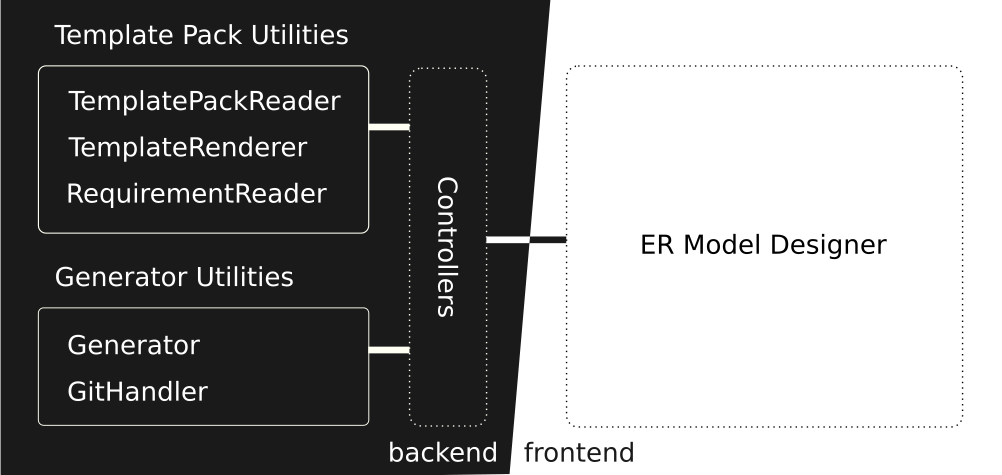
\includegraphics[width=\textwidth]{contents/images/components.png}
		\caption{A rendszer fontosabb elemei}
		\label{fig:components}
	\end{figure}

	Az előző irányelvek szerint a rendszer fontosabb elemei a fenti ábrán láthatóak. Az ábra két részből áll. A backend és a frontend. A frontend a felhasználói felületet biztosító része a programnak, a backend pedig a felhasználói felülettől jövő kérések feldolgozásáért felelős. A kérést elsőnek egy Router kapja meg, ami a megfelelő Controller-hez irányítja azt. A Controller megvalósítja a kérés feldolgozását az erre specializálódott osztályok segítségével, és visszatér egy válasszal, ami megjelenik a felhasználói felületen. 


\end{justify}
\newpage
\section{Felhasznált technológiák}
\subsection{Technológia kiválasztása az eszköz elkészítéséhez}

\begin{justify}

	A web alapú alkalmazások minden nagyobb platformon elérhetőek kompatibilitási problémák nélkül. A web a felhasználói felületre számos lehetőséget kínál, és ezek mindegyikét egyszerűen el lehet érni. Köszönhetően a Konva.js könyvtárnak már a HTMLCanvasElement-re való rajzolás is leegyszerűsödött, így a ER modell rajzolására is megfelelő választás. Nem meglepő tehát, hogy a felhasználó felület webes felületen készült. 

	A felhasználó felület programozása olyan problémákat vet fel, amikre nem érdemes saját megoldást adni, habár az egyedi implementáció általában gyorsabb programot eredményez. Ezeket a problémákat küszöbölik ki a frontend keretrendszerek. A frontend keretrendszerek közül a legelterjedtebb a facebook által kifejlesztett React. A React a nevéből adódóan reaktív keretrendszer, azaz, ha frissül az állapot, frissül a nézet is automatikusan. A React szemlélete, hogy minden egyes elemnek külön komponenst hozzunk létre. A komponensek tartalmazhatnak több komponenst is. Minden komponensnek lehet egy saját állapota és több paramétere, így látszólag egy react-es komponens ugyanolyan, mint egy HTML DOM elem, így a HTML kontextusában kényelmesen lehet használni.

	A HTML DOM egy fa szerkezet. A legtöbb frontend keretrendszer ezt a szerkezetet használja az állapot változás utáni frissítéshez. A DOM strukturálisan nem tud tartalmazni általánosabb gráfot, mint például az ER modellt. Így az speciális megoldást igényel. A Vue és az Angular túl sok mindent rejt el a tényleges implementációból, így azokban ezt a speciális igényt beeszközölni nehéz lett volna. Mivel a React rejt el a legkevesebbet, így az a megfelelő keretrendszer erre a problémakörre.

	Az alkalmazás kezelni fogja a fájlrendszert és a git-et, így teljesen web alapú nem lehet. Ahhoz, hogy a frontend-et megjeleníthessük asztali alkalmazásként, szükség van az Electron-ra. Az Electron egy NodeJS csomag, ami tartalmazza a Chromium böngésző egy részét, és gyakorlatilag ez adja a megjelenést. Az Electron miatt szükség van NodeJS-re, így a backend logikája is JavaScript lesz.

	A közös nyelv előnye, hogy bizonyos osztályokat egyaránt használhatunk a felhasználói felületen és a backend-en is. Így egy közös modell réteggel, biztosítani lehet kommunikációs interfészeket a két réteg között. 

	Mindkét réteg az ECMAScript 2018-as szabvánnyal íródott. Ezt a szabványt nem támogatja sem a NodeJS, sem a Chromium, ezért szükséges egy fordítóra, ami egyszerű JavaScript-re fordítja a kódot. A fordítást egy még nem annyira elterjedt fordító végzi: A Sucrase. A Sucrase az elterjedt Babel fordítónak egy gyorsabb és egyszerűbb alternatívája. A React esetében célszerű a JSX szabvány is, amit szintén a Sucrase fordít javascriptre. A JSX lehetővé teszi, hogy a react-es komponenseket írhassuk html elemként.


\end{justify}
\newpage
\subsection{Felhasznált saját külső könyvtárak}
\subsubsection{Bevezetés}

\begin{justify}

	A fejlesztés során sok olyan könyvtárat meg kellett írni, ami eddig nem volt még elérhető, de érdemes lehet felhasználni egy másik projektben is. Mivel NodeJS-ben készült a szoftver, a Node Package Manager segítségével publikálhatóak saját könyvtárak is.


\end{justify}
\newpage
\subsubsection{Vecjs - Két dimenziós vektor számításokért felelős könyvtár}

\begin{justify}

    A felhasználói felület vektorgrafikai számításaihoz szükséges egy gyors két dimenziós függvény könyvtár. A könyvtár vecjs néven érhető el (https://www.npmjs.com/package/vecjs). A vecjs a leggyakoribb vektor műveleteket tartalmazza funkcionális paradigmákkal. 
    
    Az eddig is meglévő vektor műveleteket segítő könyvtárak nem voltak alkalmasak átlátható kód írására. A legtöbb mutable volt, ami azt jelenti, hogy a művelet módosította a változót, és nem újat adott vissza. Pl.:

	\begin{lstlisting}[language=javascript]
	a = new Vec2D(10,20)
	b = new Vec2D(30,40)
	a.add(b)
	\end{lstlisting}

	Ekkor az $ a $ értéke: $ Vec2D(40,60) $. A probléma ezzel az, hogy az $ a $ eredeti értékét nem érjük el a hozzáadást követően. Matematikai problémáknál jobb megoldás, ha a változók nem módosulnak. Pl.:

	\begin{lstlisting}[language=javascript]
	a = new Vec2D(10,20)
	b = new Vec2D(30,40)
	c = a.add(b)
	\end{lstlisting}

	Ebben az esetben a $ c $ kapja meg az $ a + b $ értékét, de itt az $ add $ függvény nem módosítja a bemenet értékét. Az implementáció lehetővé teszi, hogy a megszokott infix jelölésként alkalmazzuk az összeadást. Pl.:

	\begin{lstlisting}[language=javascript]
	(a) .add (b) .add (c)
	\end{lstlisting}

\end{justify}
\newpage
\subsubsection{React-konva-anchors - Dinamikus pozicionálást és méretezést segítő könyvtár a react-konva számára}

\begin{justify}

	A Konva egy canvas-re rajzolást leegyszerűsítő könyvtár, amit ha nagy projektnél használunk, akkor érdemes valamilyen frontend keretrendszerrel egybekötni. A kettő könyvtár közötti kapcsolatot - egy másik - a react-konva biztosítja. A react-konva-anchors segítségével definiálhatunk elemek közti relatív elhelyezést és méretezést, ami automatikusan frissül, ha a referencia elem is frissül. 

	A cél az volt, hogy a CSS-hez hasonló logikával lehessen megoldani a pozicionálást, de az eredmény egy sokkal általánosabb megoldás lett. Tegyük fel van két elemünk. Az egyik egy téglalap, aminek az origója a téglalap bal felső sarkában van. A másik egy kör, aminek az origója a kör közepén van. Legyen a cél az, hogy a kört a téglalap jobb felső részére szeretnénk tenni. Szeretnénk azt is elérni, hogyha változik a téglalap szélessége akkor a kör pozíciója is frissüljön. A megoldáshoz szükség van megadni a mozgatni kívánt elem origóját relatívan. A relatív origó a \ref{fig:position_anchor}. ábra szerint számolódik.

    \begin{figure}[h]
        \centering
		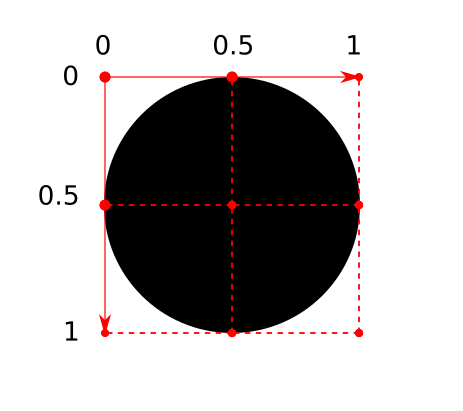
\includegraphics[width=10cm]{contents/images/position_anchor.png}
		\caption{ Egy kör relatív koordinátarendszere}
		\label{fig:position_anchor}
	\end{figure}

	Így tehát az $ (0.5,0.5) $ lesz a kör origója. Az origót ezután átállíthatjuk, ha esetleg nem a közepe szerint szeretnénk mozgatni, de mivel nekünk jó a közepe, ezért marad a $ (0.5,0.5) $. A referencia elemnél hasonlóan meg kell adnia az elem eredeti origóját relatívan, ezután ott is átállíthatjuk a kívánt helyre. Jelen esetben a referencia origója $ (0,0) $. Mivel mi a jobb felső sarokba szeretnénk mozgatni a kört, ezért ezt az origót átállítjuk $(1,0)$-ra. A horgony úgy működik, hogy az elemet eltolja a referencia elemhez úgy, hogy a két elem origója megegyezzen, így megvalósítva a százalékos elhelyezést. Szükség lehet egy utólagos nem százalékos eltolásra is (pl.: $(10px,-10px)$). Erre az esetre itt egy példakód:

	\begin{lstlisting}[language=jsx]
	<PositionAnchor 
	element={() => ELEMENT_TO_MOVE}
	elementOrigin={{x:0.5,y:0.5}}
	elementDesiredOrigin={{x:0.5, y:0.5}}

	reference={() => REFERENCE_ELEMENT}
	referenceOrigin={{x:0,y:0}}
	referenceDesiredOrigin={{x:1, y:0}}

	shift={{x:-25, y:0}}
	change={(x, y) => this.setState({ POS: { x, y } })} />
	\end{lstlisting}

	A $PositionAnchor$-t lehet használni egy elem saját magának az eltolására is. Például, ha egy téglalap origója a $(0,0)$-ban van, a téglalap pozíciója szintén $(0,0)$, de mi szeretnénk az origóját megváltoztatni $(0.5,0.5)$-re azért, hogy a koordináta-rendszerben a $(0,0)$ pont legyen a téglalap közepe. Erre azonban túl bonyolultnak tűnhet a $PositionAnchor$. Ezért van egy specifikusabb változata: a CenterAnchor.

	\begin{lstlisting}[language=jsx]
	<CenterAnchor
	element={() => ELEMENT_TO_CENTER}
	change={(x, y) => this.setState({ POS: { x, y } })} />
	\end{lstlisting}

	Mivel a $PositionAnchor$ elég általános ahhoz, hogy mindenféle pozicionálást meg lehessen vele oldani, és a CenterAnchor segítségével a középre helyezés is leegyszerűsödött, ezért a pozicionáláshoz nem kell több horgony elem. A méret kezeléséhez viszont igen. Legsűrűbben a szélességet kell horgonyozni valamilyen referencia elem méretéhez. Például egy téglalap méretét a benne lévő szöveg méretéhez. Erre szolgál a $WidthAnchor$.

	\begin{lstlisting}[language=jsx]
	<WidthAnchor
	reference={() => REF_ELEMENT}
	element={() => ELEMENT_TO_RESIZE}
	padding={25}
	change={width => this.setState({EL_W: width })} />
	\end{lstlisting}

	A $WidthAnchor$ a megadott referencia elem méretét leolvassa, és az elemet átméretezi úgy, hogy a padding értékét hozzáadja a mérethez. Minden esetet viszont lehetetlen lenne lefedni speciális horgonyokkal, ezért van a $CustomAnchor$, ami lehetőséget nyit saját megoldásokra is.

	\begin{lstlisting}[language=jsx]
	<CustomAnchor 
	reference={ () => EL_TO_WATCH }
	element={ () => EL_TO_CHANGE }
	result={ (ref) => ({ x: ref.width(), y:0 }) }
	isUpdateNeeded={
		(el, res) => 
		el.x() !== res.x || el.y() !== res.y 
		}
        change={(res)=> { this.setState({PROP: res }) } 
    } />
	\end{lstlisting}

	A $CustomAnchor$ esetében szükséges definiálni azt, hogy mikor frissítse az elemet, ezzel el lehet kerülni azt, hogy egy állandó frissítési ciklus alakuljon ki, amiatt, hogy egy horgony referencia eleme egy horgony módosítandó eleme. Meg kell adni a számítást, amit egy függvényben, kell megvalósítani.

\end{justify}

\newpage
\subsubsection{FastEJS - EJS-hez hasonló sablonmotor}

\begin{justify}

	Az EJS egy ismert egyszerű sablonmotor a javascript nyelvhez. A FastEJS ennek egy gyorsabb és használhatóbb implementációja. A fő ok, amiért nem volt jó az EJS az, hogy EJS-hez hasonló sablonokat is szükséges lehet generálni, azaz a sablon sablonját is meg kell írni. Az EJS erre lehetőséget nem adott, vagy csak hibásan. Az implementáció egyszerű reguláris kifejezéseket tartalmaz, és egy eval kifejezést. A regexp összeállítja a sablonból a javascriptet, az eval (evaluate) pedig lefuttatja azt.

	Mivel a javascript interpretált nyelv, ezért az egész sablon motort szabadon össze lehet állítani szövegesen. Ez lehetővé teszi, hogy az egyes regexp utasítások kikapcsolhatóak legyenek. Példa a motor lehetséges regexp utasításaira:

	\begin{lstlisting}[language=javascript]
	{
		"begin": ".replace(/\\n/g, '\\uffff')",
		"<%=": ".replace(/<%=([^%]+) %>/g, '`; __out += $1 + `')",
		"<%#": ".replace(/<%#([^%]+) %>/g, '')",
		"<% ": ".replace(/<%(\\s|\\uffff)/g, '`; ')",
		" %>": ".replace(/(\\s|\\uffff)%>/g, '; __out +=`')",
		"<%%": ".replace(/<%%/g, '<%')",
		"%%>": ".replace(/%%>/g, '%>')",
		"end": ".replace(/\\uffff/g, '\\n')"
	}
	\end{lstlisting}

	Mivel ez egy javascript objektum, és a könyvtár engedi a publikus hozzáférést, ezért ezek az elemek az importálás során szabadon törölhetőek. Így akár a legegyszerűbb sablonmotorrá is átalakíthatjuk, ami jelentős sebesség növekedést eredményez. Ugyanakkor lehetőséget ad új kifejezés hozzáadására vagy kifejezés módosítására is. Egy lehetséges példa a kifejezés törlésére:

	\begin{lstlisting}[language=javascript]
	const FastEJS = require('fastejs')
	delete FastEJS.tags['<% ']
	delete FastEJS.tags['<%#']
	delete FastEJS.tags['<%%']
	delete FastEJS.tags['%%>']
	delete FastEJS.tags[' %>']
	FastEJS.parse(`<%= "hello world" %>`)
	\end{lstlisting}

\end{justify}

\newpage
\section{Sablonok megvalósítása}
\subsection{Bevezetés}

\begin{justify}

	A sablonok jelentik a lelkét a generátornak. Ha nincs sablon, nincs mit generálnia. A sablon megvalósításának nagyon egyszerű folyamatnak kell lennie. Ideálisan egy fájl sablonja annyira komplex, mint maga a fájl létrehozása. Így elérhető lenne, hogy közvetlen fejlesztés helyett sablonok fejlesztése legyen a cél. Gyakorlatilag ennek elérése nem lehetséges, mert a sablon az általánossága miatt mindig bonyolultabb lesz, de törekedhetünk arra, hogy a sablonok bonyolultsága minimális legyen. 

\end{justify}

\newpage
\subsection{Nevek formázása}

\begin{justify}

	A sablonok bonyolultságának elkerülésére használhatunk segédosztályokat. Ilyen segédosztály a $Formatter$ is, ami a nevek formázását segíti. A programozásban elterjedtek bizonyos elnevezési konvenciók. PL: UpperCamelCase, lowerCamelCase, kebab-case, snake\_case. Az elnevezési konvenciók segítik az osztályok, a változók és egyéb típusú nevek megkülönböztetését. A $Formatter$ egy reguláris kifejezés segítségével alakítja át bármelyik formátumról a megadott formátumra. 

	Nem csak a kis- és nagybetű közti alakítás szükséges, hanem egyes- és többesszám közti átváltást is el kell végezni. Például egy bejegyzés entitásból generált listázás oldalnak a címe valószínűleg bejegyzések lesz. Ezzel szemben, a $Formatter$ csak angol kifejezéseket tud átalakítani, ugyanis a programkódban nincs szükség más nyelvű kifejezésekre. Ha a program más nyelvű lesz, azt lokalizációval szokták megoldani. A több szavas kifejezéseknél, az átalakítás csak az utolsó szóra vonatkozik (PL: UserRight-ból lesz UserRights). Ezt az átalakítást a Pluralize nevű NodeJS csomag végzi.

\end{justify}

\newpage
\subsection{Sablon csomagok}

\begin{justify}

	Minden fejlesztőnek megvan a saját kódstílusa, emellett a beépített sablonok kiegészítése és felülírása kulcsfontosságú, ezért a program biztosít lehetőséget saját sablonok hozzáadására és a meglévők módosítására. Az úgynevezett ``Single Source of Truth'' konvenció alapján, a program csak a felhasználói sablonokat használja. A beépített sablonokat a program a felhasználói sablonok mappájába másolja generálás előtt, ha az a mappa addig nem létezett.

	A felhasználói sablonok Linux\\GNU illetve Mac típusú rendszereken a $HOME$ környezeti változóban megadott mappát felhasználva a \lstinline[]!$HOME/.config/erscaffold-packs! mappában érhetőek el. 

	A sablon csomagok rendelkeznek egyedi tulajdonságokkal, amelyek tárolásához biztosítani kell egy fájlt. Ez a fájl az index.pack.js, ami minden csomag számára kötelező. Ez írja le a csomag nevét és a benne található követelményeket.

	\begin{lstlisting}[language=javascript]
	// BASIC_PHOENIX/index.pack.js
	const pack = {
		name: 'Basic Phoenix',
		requirements: [
			{
				file: 'resource_new.requirement.js'
			},
			// ...
		]
	};
	\end{lstlisting}

	A kiolvasását a NodeJS végzi el. Első lépésként a program beolvassa a fájl tartalmát. Mivel a javascript interpretált nyelv, ezért ad lehetőséget arra is, hogy build nélkül le lehessen futtatni a beolvasott kódot. A beolvasott kódhoz hozzáilleszti a kiolvasni kívánt változó nevét, és ezzel együtt lefuttatva, megkaphatjuk annak a változónak az értékét. Ebben az esetben a pack változó lesz a kimeneten.  

\end{justify}

\newpage
\subsection{Követelményfájlok}

\begin{justify}

	Minden sabloncsomag megoldást nyújt bizonyos követelményekre (pl: lehessen erőforrást listázni). Egy követelményen belül lehetnek kisebb követelmények is (pl: legyen új hozzáadása gomb). Ezeket a követelményeket ún. követelményfájlokban tároljuk. 

	\begin{lstlisting}[language=javascript]
	// BASIC_PHOENIX/resource_edit.requirement.js
	const requirement = {
		name: 'Edit resource',
		template: './template/edit.template.ejs',
		data(entity) {
			return entity;
		},
		children: [{ file: 'edit_go_back_button.requirement.js' }]
	};
	\end{lstlisting}

	A követelményfájlok tartalmazzák a követelmény nevét, ami majd megjelenik a kezelőfelületen a követelmények kiválasztásakor. Ezen felül tartalmazniuk kell egy kezdő sablont, ami ezen követelmény teljesítésére szolgál.

	Minden követelményfájl tartalmaz egy data nevű függvényt, ami megkap egy entitást a generáláskor. Ezzel a függvénnyel, a követelményfájl kiválaszthatja, hogy milyen adatokat kell megkapnia a beállított kezdősablonnak. 

	Ezen felül a children nevű tömb tárolja az ezen követelmény alá tartozó követelményeket. 

	Későbbi továbbfejlesztésekben a gyerek követelmények tárolása helyett, szülő követelmény megadása lesz a kötelező, ezzel modulárisabbá lehet tenni a rendszert. Ezzel a megoldással elérhető lesz, hogy egy sabloncsomag egy másik sabloncsomagot egészíthessen ki. Az, hogy milyen további követelményeket választhatunk ki az függhet az entitástól, ezért későbbiekben lesz egy függvény, ami a követelmény paramétereit fogja visszaadni egy bemeneti entitásból. 

\end{justify}

\newpage
\subsection{Sablonok}

\begin{justify}

	A sablonoknak két fajtája van. Az egyik típus az amelyik létrehoz fájlokat. A másik amelyik kiegészíti a már létrehozottakat.

	\begin{lstlisting}[language=ejs]
	<%
	// BASIC_PHOENIX/view/view.template.ejs

	let app_name = Formatter.snakeCase(APPNAME)
	let AppName = Formatter.upperCamelCase(APPNAME)
	let entity_name = Formatter.snakeCase(entity.name)
	let EntityName = Formatter.upperCamelCase(entity.name)
	let meta = { creates: {
        fileName: "lib/"  +  app_name +  "_web/views/" 
                              +  entity_name + "_view.ex"
	}}
	%>
	defmodule <%= AppName %>Web.<%= EntityName %>View do
	use <%= AppName %>Web, :view
	end
	\end{lstlisting}

	Egy példa kimenet a fenti sablonra: 

	\begin{lstlisting}[language=elixir]
	defmodule BlogWeb.PostView do
	use BlogWeb, :view
	end
	\end{lstlisting}

	Minden sablon tartalmaz egy meta nevű változót. A meta leírja a sablon generáláshoz szükséges adatokat (pl: a létrehozandó fájl elérési útja). Minden sablon a saját fejlesztésű FastEJS sablon motort használja, amivel könnyedén kilehet nyerni a rendereléskor felhasznált változókat, így a meta objektumot is. 
    \newpage
	A kiegészítő sablonoknál a meta értéke nem csak a fájl elhelyezkedését kell, hogy tartalmazza.

	\begin{lstlisting}[language=ejs]
<%
// BASIC_PHOENIX/controller/action_show.template.ejs 
let CtxName = Formatter.upperCamelCase(entity.context)
let app_name = Formatter.snakeCase(APPNAME)
let entity_name = Formatter.snakeCase(entity.name)

let meta = { extends: {
	fileName: CONTROLLERS_FOLDER + entity_name  + "_controller.ex",
	section: "# methods",
	place: "after"
}, depends_on: [
    {template: "./controller.template.ejs", data: {entity}}
] }
%> 
def show(conn, %{"id" => id}) do
<%= entity_name %> = <%= CtxName %>.get_<%= entity_name %>!(id)
render(conn, "show.html", <%= entity_name %>: <%= entity_name %>)
end
	\end{lstlisting}

	A fenti példasablon egy controller kiegészítése egy show nevű metódussal. A meta tartalmában az $extends$ nevű objektum hívja fel a figyelmét a generátornak, hogy ez a sablon, egy másik kiegészítése. Ezen belül meg kell mondani, hogy melyik sablonfájl által generált fájlt egészítse ki, és hogy hova tegye a generált kódot a fájlon belül. A pozíció kijelölésére két paraméter szolgál. A $section$ és a $place$. A section lehet egy reguláris kifejezés, illetve egyszerű szöveg típusú is. Ez mondja meg, hogy a kiegészítendő fájlban milyen kifejezést keressen. A $place$ megmondja, hogy a kiegészítés milyen elhelyezésű legyen a megtalált kifejezéshez képest.

	Egy példa kimenet a fenti sablonra: 

	\begin{lstlisting}[language=elixir]
	def show(conn, %{"id" => id}) do
	post = posts.get_post!(id)
	render(conn, "show.html", post: post)
	end
	\end{lstlisting}

	A place értékének különböző fajtái lehetnek: 

	\begin{itemize}
		\item before
		\item after
		\item replace
	\end{itemize}

	A $before$ esetében a kiegészítés a megtalált kifejezés sora előtti sorba, az $after$ esetében a megtalált kifejezés sora utáni sorba fogja helyezni a lerenderelt kiegészítő sablon tartalmát.

	Lehetőség van a megtalált kifejezés cseréjére is a $replace$ érték által. Ez esetben a megtalált kifejezés helyett a lerenderelt kiegészítő sablon tartalma fog bekerülni.

	Későbbi továbbfejlesztés során a kiegészítő sablonok át fognak alakulni, ugyanis a megtalált kifejezéstől függhet a kiegészítésnek szánt tartalom és annak elhelyezése is. Jelenleg minden típusú kifejezésre, elhelyezésre külön sablont kell létrehozni, ami növelheti a sabloncsomag átláthatóságát, viszont előfordulhat, hogy ezen sablonok közötti különbség kicsinysége miatt egyszerűbb lenne egy sablonba tömöríteni.

\end{justify}

\newpage
\section{A Tervezőfelület megvalósítása}

\begin{justify}
	\begin{figure}[H]
		\includegraphics[width=\textwidth]{contents/images/viewport.png}
		\caption{Az ER modell tervezőfelülete}
		\label{fig:viewport}
	\end{figure}

	A tervező felületnél figyelembe kellett venni, hogy ne legyen sok panel. A sok panel kitakarja a felhasználók számára érdekelt részt, a modellt. A képernyőn ezért csak alul van egy csík, ami tényleg a lehető legfontosabb elemeket tartalmazza.


	\begin{figure}[H]
		\includegraphics[width=\textwidth]{contents/images/guide.png}
		\caption{Útmutató}
		\label{fig:guide}
	\end{figure}

	A tervező a felhasználó interakciójára várva, előbb egy használati útmutatót ad. Az útmutató eltűnik, amint a felhasználó odahúzza az egér mutatóját. Az útmutató egyértelműsíti a program használatát. 
\end{justify}

\newpage

\begin{figure}[H]
	\includegraphics[width=\textwidth]{contents/images/requirements.png}
	\caption{A követelmények kiválasztása}
	\label{fig:requirements}
\end{figure}

\begin{justify}
	A generálás előtt egy sablon kiválasztási felület ugrik fel. A kiválasztás egy fa szerkezetet mutat a sabloncsomag követelményfájljai alapján.

	Jelenleg a generátor működéséből következően minden követelményfájl megkap egy entitást, ezért minden entitásra külön-külön ki kell választani a követelményeket. Későbbi továbbfejlesztési lehetőség, hogy lehetnek majd olyan követelmények is, amelyek nem igényelnek entitásokat. Ilyen követelményeket jelenleg is létre lehet hozni úgy, hogy a követelmény $data$ nevű függvénye minden entitásra ugyan-olyan értékkel tér vissza. Ekkor a követelményhez tartozó sablonok csak egyszer generálódnak le, nem pedig minden entitásra külön. Habár használható, nem tűnik jó megoldásnak, és a tervező felületen is okozhat félreértéseket.

\end{justify}

\clearpage
\section{Hozzájárulás a fejlesztéshez}
\begin{justify}
	Egy szoftver fenntartása elengedhetetlen. Előfordulhatnak egyes nem előre látható hibák, amelyek kijavítása szükséges a későbbiekben is. Emellett az integrálható funkcióknak nincs határa, és egy kódgenerátor csak jobb lehet, ha többet tud segíteni. Egy ekkora méretű szoftvert nehéz egyedüli személyként karbantartani és egyben továbbfejleszteni is. Éppen ezért a szoftver nyílt forráskódú, és bárki számára ingyenes. Az alkalmazás teljes állománya megtalálható a https://github.com/fxdave/erscaffold címen.
\end{justify}

\newpage
\pagestyle{empty}
\setcounter{secnumdepth}{0}
\sectionfont{\rmfamily\bfseries\itshape\large}
%\renewcommand{\bibsection}{\section*{Irodalomjegyzék}}
%\renewcommand{\bibname}{\textbf{\textit{Irodalomjegyzék}}}
\begin{thebibliography}{99}

	\bibitem{book:example_er_attr}
		Fogarassyné Vathy Ágnes (2017)
		{\em Adatbáziskezelő rendszerek I. - Egyed-kapcsolat modell}

	\bibitem{website:cms_or_fw}
		https://www.web-and-development.com/a-framework-or-a-cms-what-is-better-to-choose/
		(letöltés dátuma 2019. május 10.)
		{\em A Framework or a CMS? What is better to choose? | Web and Development}

	\bibitem{website:example_of_er}
		https://medium.com/omarelgabrys-blog/database-modeling-entity-relationship-diagram-part-5-352c5a8859e5
		(letöltés dátuma 2019. május 10.)
		{\em Database — Modeling : Entity Relationship Diagram (ERD) (Part 5)}

	\bibitem{website:dependency_injection}
		http://dillonbuchanan.com/programming/dependency-injection-constructor-vs-property/
		(letöltés dátuma 2019. május 10.)
		{\em Dependency Injection: Constructor vs Property}

	\bibitem{book:replace_component}
		Ivica Crnkovic, Magnus Larsson (2000)
		{\em Managing Standard Components in Large Software Systems}

	\bibitem{website:rapid_prototype}
		https://www.justinmind.com/blog/rapid-prototyping-isnt-helpful-or-is-it
		(letöltés dátuma 2019. május 10.)
		{\em Rapid prototyping isn’t helpful. Or is it? - Justinmind}

    \bibitem{website:most_known_language}
        https://insights.stackoverflow.com/survey/2018
        (letöltés dátuma 2019. május 10.)
        {\em Developer Survey Results 2018}

	\bibitem{website:component_based_development}
		https://www.techopedia.com/definition/31002/component-based-development-cbd
		(letöltés dátuma 2019. május 10.)
		{\em What is Component-Based Development (CBD)? - Definition from Techopedia}

	\bibitem{website:dependency_injection_procedural}
		https://www.quora.com/What-is-dependency-injection-How-is-it-better-than-procedural-code-if-better-Why-should-I-care
		(letöltés dátuma 2019. május 10.)
		{\em What is dependency injection? How is it better than procedural code (if better)? Why should I care? - Quora}

	\bibitem{website:coding_standards_matter}
		https://blog.fossasia.org/why-coding-standards-matter/
		(letöltés dátuma 2019. május 10.)
		{\em Why Coding Standards Matter | blog.fossasia.org}

	\bibitem{website:dependency_injection_without_container}
		https://hackernoon.com/you-dont-need-a-dependency-injection-container-10a5d4a5f878
		(letöltés dátuma 2019. május 10.)
		{\em You Don’t Need a Dependency Injection Container - Hacker Noon}


\end{thebibliography}

\newpage

\sectionfont{\rmfamily\bfseries\large}
\thispagestyle{empty}
\section{CD melléklet}

A szakdolgozat CD mellékletének könyvtárszerkezete:

% itt a csel a [], amivel nem rak ki pontokat a latex
\begin{itemize}
	\item[] /szakdolgozat.pdf
	\item[] /szakdolgozat-forraskod
	\item[] /rendszer-forraskod
	\item[] /internetes-hivatkozasok
        \begin{itemize}
            \item[] A Framework or a CMS What is better to choose Web and Development.html
            \item[] Database Modeling Entity Relationship Diagram ERD Part 5.html
            \item[] Dependency Injection Constructor vs Property.html
            \item[] Rapid prototyping in the software development life cycle Justinmind.html
            \item[] Stack Overflow Developer Survey 2018.html
            \item[] What is Component Based Development CBD Definition from Techopedia.html
            \item[] What is dependency injection How is it better than procedural code if better Why should I care Quora.html
            \item[] Why Coding Standards Matter blog.fossasia.org.html
            \item[] You Dont Need a Dependency Injection Container Hacker Noon.html
		\end{itemize}
\end{itemize}

\end{document}
